\section{Introduction}

The purpose of the work presented herein is to create a means of introducing uncertainty into deterministic models with performance superior to stand-alone Monte Carlo-based sampling techniques.

In the course of developing this material several spreadsheet-based models are analyzed. (See Appendix). A situation believed to be common is that spreadsheet-based models tend to be resistent to structural changes and their sensitivity to inputs is difficult to measure without external tools. 

A remedy of the spreadsheet-based modeling issue is to reverse-engineer the spreadsheet to discover the specific model and re-implement this model in a traditional programming environment. This re-implementation process itself only addresses the issue of model brittleness and not the sensitivity issue. The work discussed in this paper recommends implementing a class of models such as those that may be implemented in a spreadsheet environment into a special environment. The environment proposed is called \emph{RICO}, an achronym for \emph{Random input, Correlated output}.

A RICO programming environment allows the programmatic manipulation of random variables as first class computing objects. The practical upshot is that if a given model accepts numeric data, that same model implemented in a RICO environment can substitute any input value with a random variable thereby allowing the study of model input sensisitivity and model response to input uncertainty. When multiple model inputs are replaced with random variables versions of these variables may become correlated within the model even if independent initially. Numeric model outputs may then be a joint distribution of correlated random variables. 

A RICO programming environment is not a specific software product, but a specification for constructing a software programming environment. While developing RICO a collection of software modules are constructed and used to produce many of the numeric and graphical results discussed in this paper. Collectively these software modules consitute a \emph{reference} implementation of RICO. Any code snippets shown all run in at least one of the software modules within the RICO reference implementation.

Not limited to models implementable within a spreadsheet-based environment, RICO defines a number of basic mathematical operations and program flow control statements that are common to a wide variety of models. These operations include addition, subtraction, multiplication, division, exponentiation (both $x^y$ and $exp(x)$) and logarithm. Program flow control statements include conditional statements such as $IF(X \le Y)$ where either or both $X$ and $Y$ are optionally random variables. Interestingly, if at least one of $X$ and $Y$ is a random variable the conditional $IF$ statement will take \emph{both} not exclusively one or the other of the two implied code paths.

The class of models implementable in a RICO environment as large and several examples are explored. Some examples detailed below energy policy analysis, business cost savings analysis and geometric Black Scholes pricing. Important modeling components include constrained optimization and linear algebra involving random variables.

\todo{Find reference (Dineen?) likening a stochastic process to a sequence of random variables}

\subsection{A Basic Model}

At its heart a RICO model is a function of some number of inputs that produces some number of output symbolically represented in figure \ref{fig:BasicModel}.

\begin{figure}
  \centering
  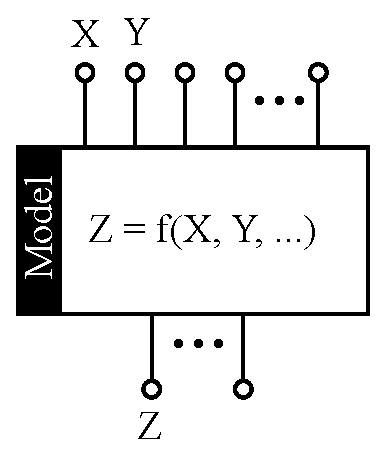
\includegraphics{Images/BasicModel.eps}
  \caption[A Basic Model]
          {A Basic Model}
  \label{fig:BasicModel}
\end{figure}

To introduce uncertainty into the model a random variable is identified for one or more inputs. As an example suppose a log-normal looking random variable $X$ such as shown in figure \ref{fig:Lognormal}.

\begin{figure}
  \centering
  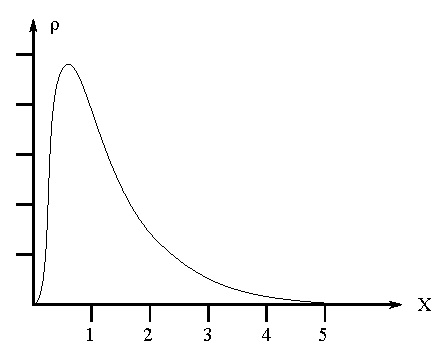
\includegraphics{Images/Lognormal.eps}
  \caption[An Input Random Variable]
          {An Input Random Variable}
  \label{fig:Lognormal}
\end{figure}

Without loss of generality suppose a basic model with a number of input variables two of which ($X$ and $Y$) are random and one output value of interest, $Z$. The Monte Carlo method of analysis requires a random sample for each random variable is generated. Suppose the random sample for $X$ is denoted $x = (x_1, x_2, ..., x_n)$ and similarly for $Y$, $y = (y_1, y_2, ..., y_n)$. The model is run $n$ times using the input values $x_i$ and $y_i$ in place of the $X$ and $Y$ inputs respectively for $i \in {1,...,n}$ generating $n$ output values for $Z$ called $z = (z_1, ..., z_n)$. 

To understand the output values $z = (z_1, ..., z_n)$ generated by an $n$-run Monte Carlo method a partition of the space of output values is created by some means and the individual $z_i$ values are counted into \emph{bins}, that is, partition intervals. A possible result with unit-interval bins is shown in figure \ref{fig:SkewedNormalHistogram}

\begin{figure}
  \centering
  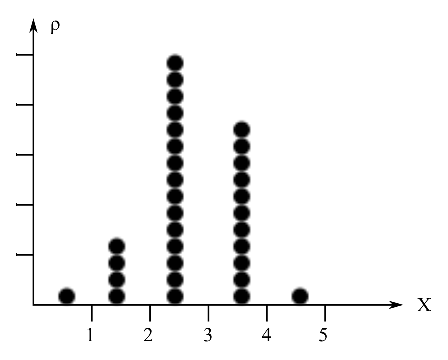
\includegraphics{Images/SkewedNormalHistogram.eps}
  \caption[Example Output Histogram]
          {Example Output Histogram}
  \label{fig:SkewedNormalHistogram}
\end{figure}

A common exercise in statistics \todo{reference} is to postulate a familiy of probability distributions and fit the `best' one to the output sample $z$. An example result is shown in figure \ref{fig:SkewedNormalFitted}

\begin{figure}
  \centering
  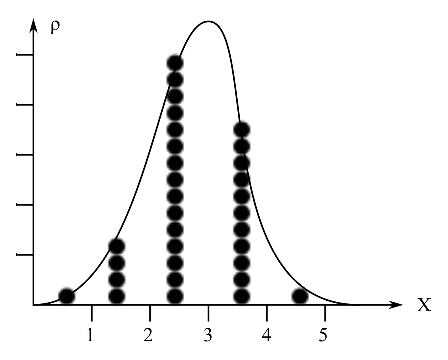
\includegraphics{Images/SkewedNormalFitted.eps}
  \caption[Example Output Histogram - Fitted]
          {Example Output Histogram - Fitted}
  \label{fig:SkewedNormalFitted}
\end{figure}

A serious concern is that in the context of an algorithmic model it is challenging to find a family of probability distributions from which to select a `best' fit for the observed output sample, $z$. If the output is unimodal a subset of the extensive exponential family may be chosen, but for multi-modal output the choice is less clear. 

The alternative offered by RICO is a hybrid approach. The RICO approach is to maintain a symbolic description of input and internal model variables where possible. When a symbolic description is not possible for an internal random variable, a numberic description is used. There is a practical limit on the number of dimensions used to describe a numeric random variable and when this limit is surpassed the final techniques applied is traditional Monte Carlo sampling.

A significant advantage that the RICO approach offers is symbolic representation of random variable tails. It is taken as axiomatic that the tail of a random variable is that region that cannot be reliably sampled. For random variables with so-called \emph{thin-tailed} probability distributions, failure to adequately sample from the tails may be inconsequential, but \emph{fat-tailed} distributions such as the Cauchy distribution have a significant amount of probability mass in the tails and this region of the support space cannot be safely ignored. Consider, for example, that the Cauchy distribution, like the St. Petersburg lottery, has no finite expected value. 

%%%%%%%%%%%%%%%%%%%%%%%%%%%%%%%%%%%%%%%%%%%%%%%%%%%%%%%%%%%%%%%%%%%%%%%%%%%%%%%%%%%%%%%%%%%

\todo{include at least one reference such as Tanner \cite{tanner96}}

